\section{Espacios de Hilbert de Kernel Reproductor (RKHS)}

Sea $H$ un espacio de Hilbert {\bf de funciones} (reales) definidas
sobre un conjunto no vacío. De este modo el espacio de Hilbert $H$
que consideramos aqu\'\i\ es un subespacio de
$\mathfrak{F}(X,\mathbb{R})=\mathbb{R}^X$:
$H\subset\mathfrak{F}(X,\mathbb{R})=\mathbb{R}^X$.
$\mathfrak{F}(X,\mathbb{R})$ denota el conjunto de funciones definidas
desde $X$ a $\mathbb{R}$.

\textbf{Nota:} $X$ eventualmente puede tener m\'as estructura si
conviene. En el contexto de las llamadas máquinas de
aprendizaje, $X$ es el espacio de las entradas a la m\'aquina y no
necesariamente es un espacio vectorial.

\begin{mydef}
En este contexto se definen los funcionales de evaluaci\'on $L_x$,
para cada punto fijo $x\in X$, sobre
$\mathfrak{F}(X,\mathbb{R})=\mathbb{R}^X$
(o sobre $H$, si se prefiere) como:
%$$
%L_x: \mathbb{R}^X\to\mathbb{R}\,,\qquad
%L_x(f):=f(x)\,,\quad\forall f\in \mathbb{R}^X\,.
%$$


\begin{eqnarray}
L_x: H &\rightarrow &\mathbb{R} \nonumber \\
 f &\rightarrow & L_x(f):= f(x) \quad\forall f\in H \label{eq:evalfu}
\end{eqnarray}

\end{mydef}


\setlength{\parskip}{5mm}
\begin{center}
\begin{tikzpicture}
   \foreach \x in {1,2,3}{
   \node[fill,circle,inner sep=5pt,scale=0.3] (d\x) at (0,\x) {};
   \node[draw=none] at (0,\x+0.3) {$f_\x$};
   }
   \node[fit=(d1) (d2) (d3),ellipse,draw,minimum width=2cm] {}; 

   \foreach \x[count=\xi] in {1,2,3}{
   \node[fill,circle,inner sep=5pt,scale=0.3] (r\xi) at (3,\x) {};
   \node[draw=none] at (3,\x+0.3) {$f_\x(x)$};
   }
   \node[fit=(r1) (r2) (r3),ellipse,draw,minimum width=2cm] {}; 

    %\draw \boundellipse;
    %\draw \secondboundellipse;
    \node[anchor=south] at (current bounding box.north) {$L_x:
    H \to \mathbb{R}$};
    \draw[-latex] (d1) -- (r1);
    \draw[-latex] (d2) -- (r2);
    \draw[-latex] (d3) -- (r3);
\end{tikzpicture}
\end{center}



\noindent \textbf{Nota:} Un funcional de evaluación $L_x$ es siempre \textbf{lineal}
ya que se cumple que:
\begin{equation*}
L_x(\alpha f + \beta g)
= (\alpha f + \beta g)(x)
= \alpha f(x) + \beta g(x)
= \alpha L_x(f) + \beta L_x(g)
\end{equation*}
para todo $\alpha,\beta\in\mathbb{K}$ y todo $f,g\in H$.


\begin{mydef}
Se dir\'a que un espacio de Hilbert $H$ es RKHS si y s\'olo si
$H$ es un espacio de funciones sobre un conjunto no vac\'\i o $X$, donde
todos los funcionales de evaluaci\'on $L_x:H\to\mathbb{R}$, $x\in X$, 
$L_x(f)=f(x)$ para todo $f\in H$, son continuos.
\end{mydef}


\noindent\textbf{Nota:} Un funcional de evaluaci\'on $L_x$, $x\in X$ fijo es
\textbf{continuo} si para una sucesi\'on de funciones $\{f_n\}$ en
$H\subset\mathfrak{F}(X,\mathbb{R})=\mathbb{R}^X$, con $f_n
\overset{\|\cdot\|}{\rightarrow}f$ para $n\rightarrow\infty$,
$|L_x(f_n-f)| \rightarrow 0$.  
La convergencia se\~nalada $f_n \overset{\|\cdot\|}{\rightarrow}f$
significa que:
\begin{equation*}
\|f_n-f\|^2 = \langle f_n-f, f_n -f \rangle \rightarrow 0
\quad\text{para}\quad n\rightarrow\infty\,.
\end{equation*}
Para que $L_x$ sea continuo debe cumplirse que:
\begin{equation}\label{stetigkeit}
|L_x(f_n-f)| = |L_x(f_n)-L_x(f)| = |f_n(x) -f(x)| \rightarrow 0 
\quad\text{para}\quad n\rightarrow\infty\,.
\end{equation}
N\'otese que los valores de $L_x$ y de $f_n,f$ est\'an en
$\mathbb{K}=\mathbb{R}$, de modo que $|\cdot|$ denota el valor absoluto
usual.
N\'otese tambi\'en que, dado que $H$ es un espacio de Hilbert,
basta considerar una sucesi\'on nula $\{f_n\}$ y $f=0$.



\subsection{Funcionales de evaluación}
¿Son continuos todos los \textbf{funcionales de evaluación} sobre un
espacio de Hilbert de funciones sobre un conjunto no vacío dado?

\textbf{Respuesta:}
La respuesta tambi\'en es NO, como se discute m\'as adelante.


%Ese mismo ejemplo se puede adaptar para exhibir un funcional lineal
%no-continuo sobre un espacio de Hilbert.
%{\color{red} Exh\'\i balo}

Aquí consideramos un conjunto no vacío $X$, un espacio de Hilbert
$H$ de funciones reales sobre $X$, es decir,
$H\subset\mathfrak{F}(X,\mathbb{R})=\mathbb{R}^X$, y fijamos un
elemento genérico $x\in X$.



\begin{enumerate}

\item ?`Es $L_x$ continuo?\quad Rpta.: No siempre. 
Damos un ejemplo de un funcional evaluaci\'on no continuo sobre un
espacio de Hilbert $H$ de funciones definidas sobre un conjunto no
vac\'\i o $X$. Por lo tanto, la condici\'on (\ref{stetigkeit}) no
siempre se cumple, como lo demuestra el siguiente contraejemplo:

\begin{itemize}
\item
Sea $x =[0,1]\subset\mathbb{R}$ y 
$$
\mathcal{H} = \left\{ f:[0,1]\rightarrow\mathbb{R} \ \mid\ 
\text{$f$ es integrable con}\ \int_0^1|f(x)|^2\,dx<\infty\right\}\,.
$$
N\'otese que las funciones $f\in\mathcal{H}$ pudieran no estar definidas
en subconjuntos de $[0,1]$ de medida nula.

\item
La medida considerada en este contra-ejemplo es la medida de Lebesgue,
que atribuye la medida $b-a$ a todo intervalo
$\mathfrak{I}\subseteq[0,1]$ con 
$0\leq a:=\inf\mathfrak{I}\leq\sup\mathfrak{I}=:b\leq1$.
N\'otese que esta definici\'on incluye todos los intervalos abiertos,
cerrados, semi-abiertos, etc.

\item
En $\mathcal{H}$ se acostumbra a identificar las funciones que
difieren a lo m\'as en subconjuntos $S$ de $[0,1]$ con medida nula.

\item
M\'as precisamente, se introduce la relaci\'on:
$$
f\sim g \quad\Leftrightarrow\quad
\int_{S(f,g)} |f(x)-g(x)|^2\,dx=0\,,\qquad f,g\in\mathcal{H}\,,
$$
donde
$$
S(f,g):=\big\{ x\in[0,1]\ \mid\ 
\text{$f(x)$ y $g(x)$ son diferentes}\;\big\}\,.
$$
N\'otese que la definici\'on de $S(f,g)$ incluye los puntos
$x\in[0,1]$ donde $f(x)$, o $g(x)$, o ambas funciones, no est\'an
definidas.

%\smallskip\noindent$\bullet$\quad
\item
La relaci\'on ``$\sim$'' es una relaci\'on de equivalencia sobre
$\mathbb{H}$. {\bf (!`Demu\'estrelo!)}

%\smallskip\noindent
\item
Entonces se define:
$$
H = \mathcal{H}/\!\!\sim\; 
= \text{conjunto cuociente de $\mathcal{H}$ 
        con respecto a la r. de eq. $\sim$}\,.
$$
%\smallskip\noindent$\bullet$\quad
TAREA: Asegurarse de entender bien qu\'e significa
$H = \mathcal{H}/\!\!\sim$. \\
Hint: Recuerde los cursos de Introducci\'on a
la Inform\'atica y Computaci\'on Cient\'\i fica.

%\smallskip\noindent
\item
$H$ es un espacio vectorial sobre $\mathbb{R}$.
TAREA: Demu\'estrelo.

%\smallskip\noindent
\item
Sobre $H$ se define el producto interno
$$
\langle f,g \rangle = \displaystyle \int_0^1 f(x)\,g(x)\,dx\,,\quad
f,g\in H\,.
$$
TAREA: Verifique que $\langle\cdot,\cdot\rangle$ satisface todos los
axiomas de un producto interno.

\item
El producto interno $\langle\cdot,\cdot\rangle$ define una norma
$\|\cdot\|$ sobre $H$ mediante:
$$
\|f\|=\big( \langle f,f\rangle \big)^{1/2}
= \left( \int_0^1|f(x)|^2\,dx \right)^{1/2}\,,\qquad f\in H\,.
$$
TAREA: Verifique que $\|\cdot\|$ satisface los axiomas de una norma
sobre un espacio vectorial.

\item
El espacio $H$ es completo con respecto a la norma $\|\cdot\|$.\\
TAREA: Verifique este aserto.

\item
En consecuencia, $(H,\langle\cdot,\cdot\rangle)$ es un espacio de
Hilbert.
En nuestro contraejemplo, evidentemente, 
$H=L_{\mathbb{R}}^2([0,1],\mathcal{B},\lambda)=$ el espacio de las
funciones reales de energ\'\i a finita definidas sobre el intervalo
$[0,1]$, con respecto a la $\sigma$-\'algebra $\mathcal{B}$ de los
conjuntos de Borel y la medida unidimensional $\lambda$ de Lebesgue.

Es necesario notar, sin embargo, que los elementos de
$H=L_{\mathbb{R}}^2([0,1],\mathcal{B},\lambda)$
son {\em clases de equivalencia $f$ de funciones\/}
$\varphi:X\to\mathbb{R}$, $\varphi\in f$, que difieren (o pueden diferir)
a lo m\'as en subconjuntos de $[0,1]$ con medida nula.

De este modo, si fijamos un $x_0\in[0,1]$, el funcional (lineal)
$L_{x_0}$ de evaluaci\'on en $x_0$ no se puede definir pues los
representantes $\varphi$ de una clase
$f\in H=L_{\mathbb{R}}^2([0,1],\mathcal{B},\lambda)$
pueden tener (!`y tienen!) valores bien diferentes en el punto $x_0$.
En otras palabras, el conjunto:
$$
\left\{ \varphi(x_0)\mid \varphi\in f \right\}\,,\quad
f\in H=L_{\mathbb{R}}^2([0,1],\mathcal{B},\lambda)\,,
$$
no necesariamente se reduce a un punto en $\mathbb{R}$ y, 
por lo tanto, en este caso {\bf no} tiene sentido escribir
$L_{x_0}(f)=\varphi(x_0)$, $\varphi\in f$.
En efecto, no sabr\'\i amos cu\'al representante $\varphi$ de $f$
elegir para calcular $L_{x_0}(f)$.

\smallskip
{\em Conclusi\'on\/}: En el caso del contraejemplo ni siquiera es
posible definir los funcionales de evaluaci\'on $L_{x_0}$,
$x_0\in[0,1]$, sobre $H=L_{\mathbb{R}}^2([0,1],\mathcal{B},\lambda)$.

\item
En casos particulares espec\'\i ficos es posible definir $L_{x_0}$.
Por ejemplo, si definimos las {\em funciones\/} (i.e., no clases
de equivalencia de funciones):
$$
\varphi_n(x):=
\begin{cases}
1-n\,x\,, & 0\leq x< 1/n\,, \\
0\,, & 1/n\leq x\leq 1\,,
\end{cases}
\quad (n\in\mathbb{N})\,,\qquad
\varphi(x):=0\quad\forall x\in[0,1]\,,
$$
entonces podemos constatar que:
(i) $\varphi,\varphi_n\in H$ para todo $n\in\mathbb{N}\,$;
(ii) $\varphi_n\to \varphi$ con respecto a la norma $\|\cdot\|$
     de $H$ para $n\to\infty$;
(iii) Para el funcional de evaluaci\'on $L_0$ en $x_0=0\in[0,1]$
      se tiene:
$$
L_0(\varphi_n)=1\ \forall n\in\mathbb{N}\quad\text{y}\quad
L_0(\varphi)=0\,.
$$
Luego, $1=L_0(\varphi_n)\not\to L_0(\varphi)=0$ en $\mathbb{R}$
para $n\to\infty$.
De consiguiente, en este caso particular\'\i simo, el funcional de
evaluaci\'on $L_0$ si bien se puede definir, resulta que no es
continuo. \\
TAREA: Demuestre todo esto.

\item
El contraejemplo precedente demuestra que no todo funcional de
evaluaci\'on en un espacio de Hilbert de funciones es continuo y,
por lo tanto la condici\'on RKHS es una genuina condici\'on que
los espacios de Hilbert, en el contexto de las m\'aquinas de
aprendizaje, deben satisfacer.
\end{itemize}
\end{enumerate}



\subsection{Consecuencias de RKHS}

\begin{enumerate}[(a)]
\item
Si $H$ es un espacio de Hilbert de funciones sobre un conjunto no
vac\'\i o $X$, todo {\color{red} \bf funcional de evaluaci\'on}
$L_{x_0}$, $x_0\in X$ fijo, es autom\'aticamente lineal.
Si $H$ adem\'as satisface la condici\'on que hemos denominado RKHS,
$L_{x_0}$ es continuo y, por el teorema de representaci\'on de Riesz,
se puede representar mediante el producto interno de $H$:
existe un \'unico vector $k_{x_0}\in H$ tal que:
\begin{equation*}
L_{x_0}(f):= f(x)= \langle f,k_{x_0}\rangle\quad\forall\,f\in H\,.
\end{equation*}

\begin{myremark}
Los p\'arrafos (b) y (c) que siguen en esta observaci\'on enmarcada
contienen varios {\bf gruesos errores} (que las lectoras deber\'an
aquilatar apropiadamente) y, por lo tanto, es mejor eliminarlos:
%verificar!!!!! pagina 32 de Smola

(b)\ $H\subset\mathcal{F}(X,\mathbb{R})
=\mathbb{R}^X=\{f:X \rightarrow \mathbb{R}\}$. 
$L_x$ es autom\'aticamente lineal y cont\'\i nuo ({\bf !`FALSO!})
para un $x$ fijo y dado que $H$ es un RKHS $L_x$ es adem\'as cont\'\i nuo.

\smallskip\noindent
\textbf{Demostraci\'on de continuidad.}\quad
{\bf !`No hay nada que demostrar pues la condici\'on RKHS garantiza
la continuidad de los funcionales de evaluaci\'on!}

Si se tiene una sucesi\'on ${f_n}$ en $H$ con:
\begin{equation}\label{eq:cont1}
f_n \rightarrow n\ \text{{\bf ?`n? !`EROR!} para } n \rightarrow \infty 
\Longleftrightarrow ||f_n-f||_H \rightarrow 0, n\rightarrow \infty
\end{equation}
se cumple en que:
\begin{equation*}
|f_n(x) - f(x) | 
= | L_x(f_n-f) | \leq ||L_x|| ||f_n-f|| \rightarrow 0, n\rightarrow \infty
\end{equation*}
Ya sabemos de la ecuaci\'on (\ref{eq:cont1}) que 
$||f_n-f||_H \rightarrow 0$ y se verifica que $||L_x||$ 
al ser cont\'\i nuo est\'a acotado por:
\begin{equation*}
||L_x|| = \sup_{f \in H,f \neq 0} \frac{|L_x(f)|}{||f||}
\end{equation*}
{\bf En realidad lo correcto ser\'\i a decir: si
$||L_x|| = \sup_{f \in H,f \neq 0} \frac{|L_x(f)|}{||f||}<\infty$,
entonces $L_x$ es continuo.}

\smallskip\noindent
(c)\ $f\in H$ es una funci\'on definida como:
\begin{eqnarray*}
f: X &\rightarrow &\mathbb{R} \\
 x &\rightarrow & f(x) 
\end{eqnarray*}
{\bf (c) es correcto pero no aporta nada nuevo.}

\smallskip\noindent
Las lectoras deben corregir estos p\'arrafos hasta darle un sentido
matem\'aticamente correcto, pero no deben ser inclu\'\i dos en la
versi\'on final del documento.
\end{myremark}

\item
la funci\'on $k_x$ se denomina \textit{kernel reproductor para el punto}
$x$. 

\item
Se denomina \textit{kernel reproductor para} $H$ a la siguiente funci\'on:
\begin{eqnarray*}
K: X \times X &\rightarrow &\mathbb{R} \\
(x,y) &\rightarrow & K(x,y):= k_x(y) = L_y(k_x) = \langle k_x,k_y\rangle\,.
\end{eqnarray*}
\end{enumerate}



%FALTA LO DE LA INMERSION

%% \begin{figure}[ht!]
%% \centering
%% \includegraphics[width=90mm]{featuremaphilbert.jpg}
%% \caption{Feature map in RKHS}
%% \label{overflow}
%% \end{figure}




\begin{figure}[htpb!]
\centering
\includegraphics[width=90mm]{img/featuremaphilbert.jpg}
\caption{Feature map in RKHS}
\label{overflow}
\end{figure}



